\documentclass[12pt]{article}
\usepackage{CJKutf8, indentfirst, graphicx, subfigure}
\begin{document}
\begin{CJK}{UTF8}{bsmi}
\title{Mid-term Project Report}
\author{Group 8 鄭余玄、謝昀佐、陳令原}
\date{}
\maketitle
\section{團隊合作}
Mid-term project 因為需要兩到三人一組,
所以我們這組決定一定要使用版本管理系統,
因此最後選擇在 GitHub 上開一個 private repo(圖 \ref{gh}),
首先是因為這是作業,所以用 private 就不會被找到,
而且如果交完作業,還可以開源讓大家來使用。

\begin{figure}[h]
  \caption{GitHub}
  \centering
  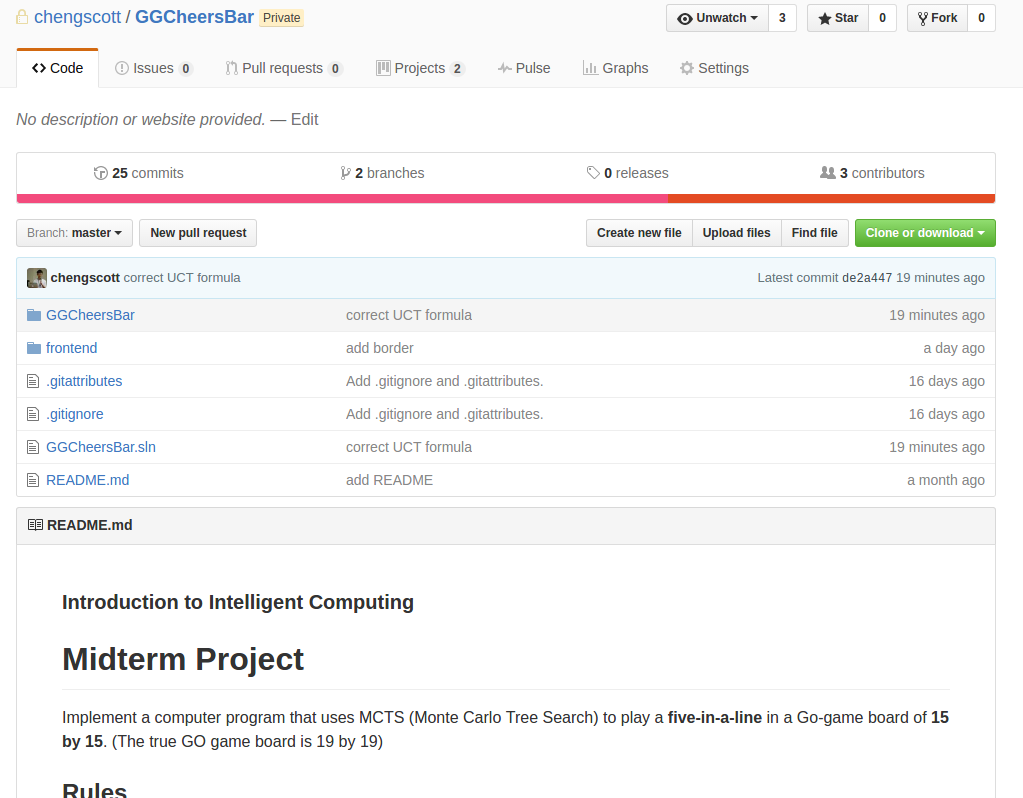
\includegraphics[width=1\textwidth]{gh}
  \label{gh}
\end{figure}


\section{理論運用}
蒙地卡羅樹狀搜尋(Monte Carlo Tree Search)會導致一種一維隨機漫步。
因為以前有組員寫過隨機漫步的經驗,所以稍唯有一些了解。
在考慮機率空間 $(\Omega, \mathcal{F}, P)$ 和可測空間 $(S, \Sigma)$ 之下,蒐集所有在拓樸空間 $T$ 中的 $X$ 隨機變數。
程式只會進行有限步運算,因此考慮有限機率測度 $S^k$,在合適的拓樸限制下,可以用相容的有限維機率分佈來定義這個隨機過程。

樹狀搜尋過程則是非常簡單,共分成 Selection、Simulation、Expansion 和 Backpropogation 四個階段。
\begin{figure*}[h]
  \caption{mcts.cpp: Line 98}
  \centering
  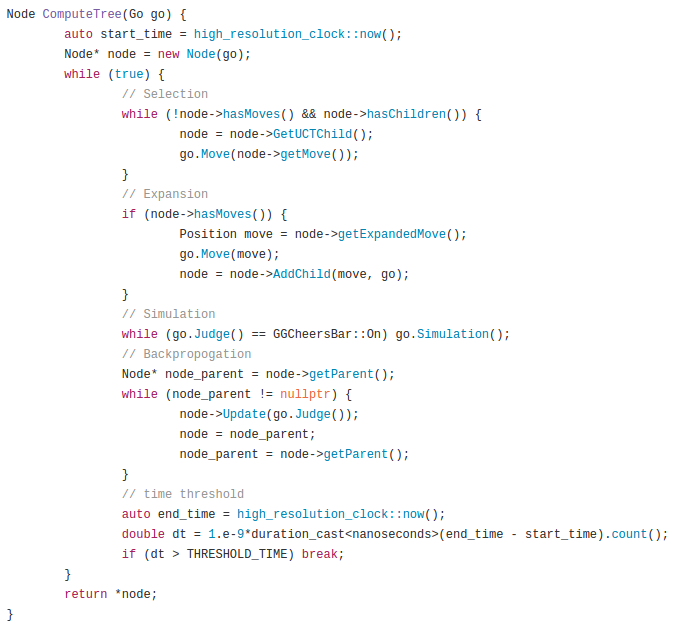
\includegraphics[width=.8\textwidth]{tree}
\end{figure*}

\section{實做過程}
因為 MCTS 是非常著重節點展開,因此我們這組選用 C/C++ 來實做核心功能,目的是為了透過越底層的指標操作,來減低計算複雜度的常數。
而棋盤顯示部份則是用 HTML5 和 JavaScript 來完成,中間藉由 websocket 和 c socket server 來建立連線。
當初構想是可以讓核心的 C 程式遠端跑在效能更到的電腦上,不過因為後來老師宣佈不能連上網路,所以也就做罷。
這套系統架構的規劃是非常有彈性的,假如今天有新的棋盤外觀模組,則只需要抽換前端即可,核心判斷程式完全照常運作。
此外,若考慮人和人或 AI 之間的連線,之需要針對中間層 socket 做適當的改變,其他部份一樣是照舊。
而且在這規劃之下,組員之間分工可以較明確。

主程式整體結構上,雖然要求效能,但是 Donald Knuth 說過,過早的優化是邪惡的,因此開發時主要是避免一些 overhead 和降低演算法複雜度。
所有物件皆有良好的封裝,也有參考一些設計模式,像是 Strategy 模式等等,以及盡量去遵守 S.O.L.I.D. 原則。
所有程式碼,像是程式變數命名、物件區塊順序等細節皆有按照 Google Coding Style,讓我們這組開發上有一致的規範。

此外,MCTS 也十分著重隨機性,從前述的理論就可以略知一二。
但是 C/C++ 所提供亂數函式庫是惡名昭彰的不隨機,因此特別選用了 C++11 提供的 mersenne twister engine(mt19937)去做隨機分佈。

\section{實驗}
就理論而言,總是聲稱某些參數被控制的況下,MCTS 則可以收斂。
但是實際上來說,那些參數往往都只能藉由猜測、嘗試或實驗而得到的。
因此,我們也對程式做了一些實驗。

通常這種搜尋樹的樣子,非常容易行程混沌系統。
一旦行成混度系統,整個系統是非常不穩定,而且非常容易崩塌(MCTS 的隨機性更是會突顯這件事)。
\begin{figure*}[h]
  \caption{搜尋樹}
  \centering
  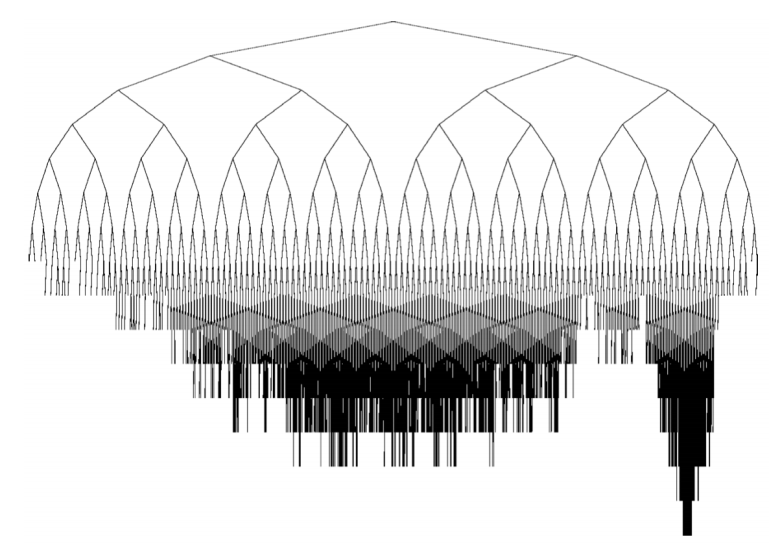
\includegraphics[width=1\textwidth]{search}
\end{figure*}
在圖 \ref{two_ai} 中,兩支 AI 會陷入一個互相防守的棋局,這就是典型的混沌系統,
\begin{figure*}[h]
  \caption{兩支 AI 對弈}
  \centering
  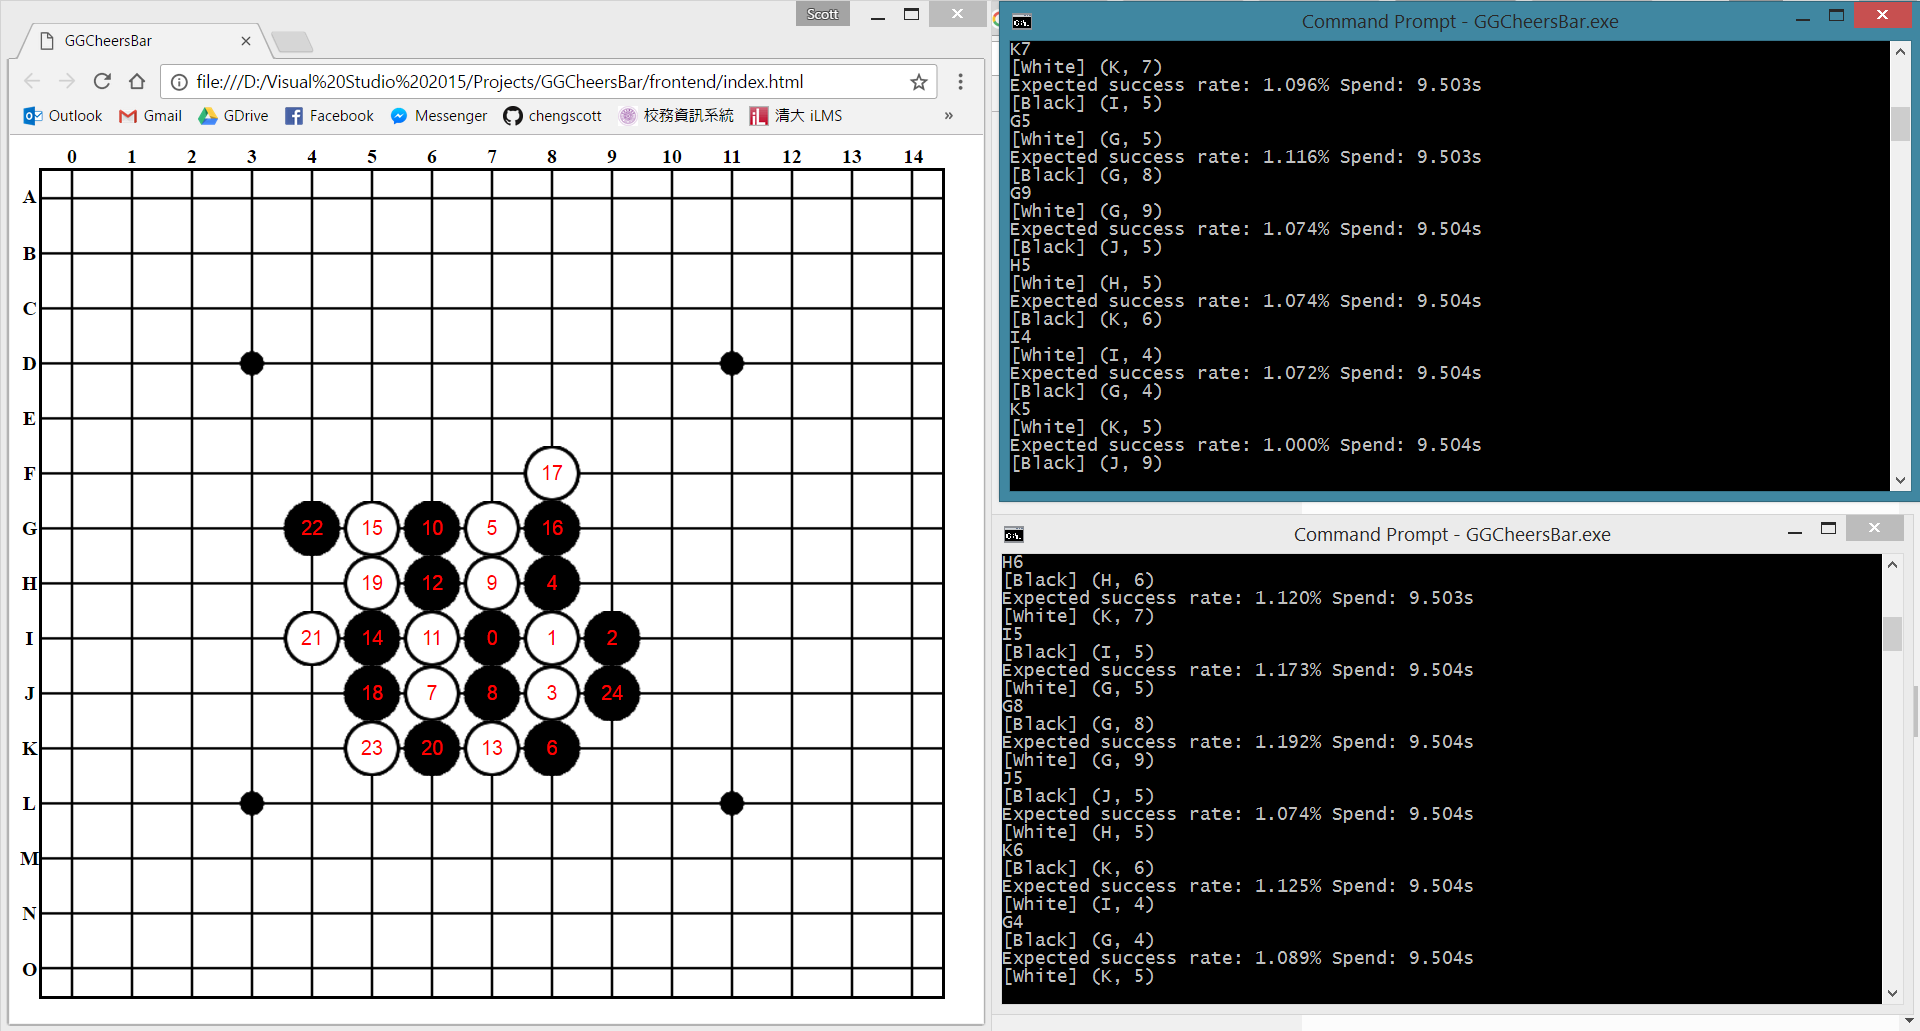
\includegraphics[width=1\textwidth]{chaos}
  \label{two_ai}
\end{figure*}

\begin{figure*}
  \caption{人工智慧}
  \centering
  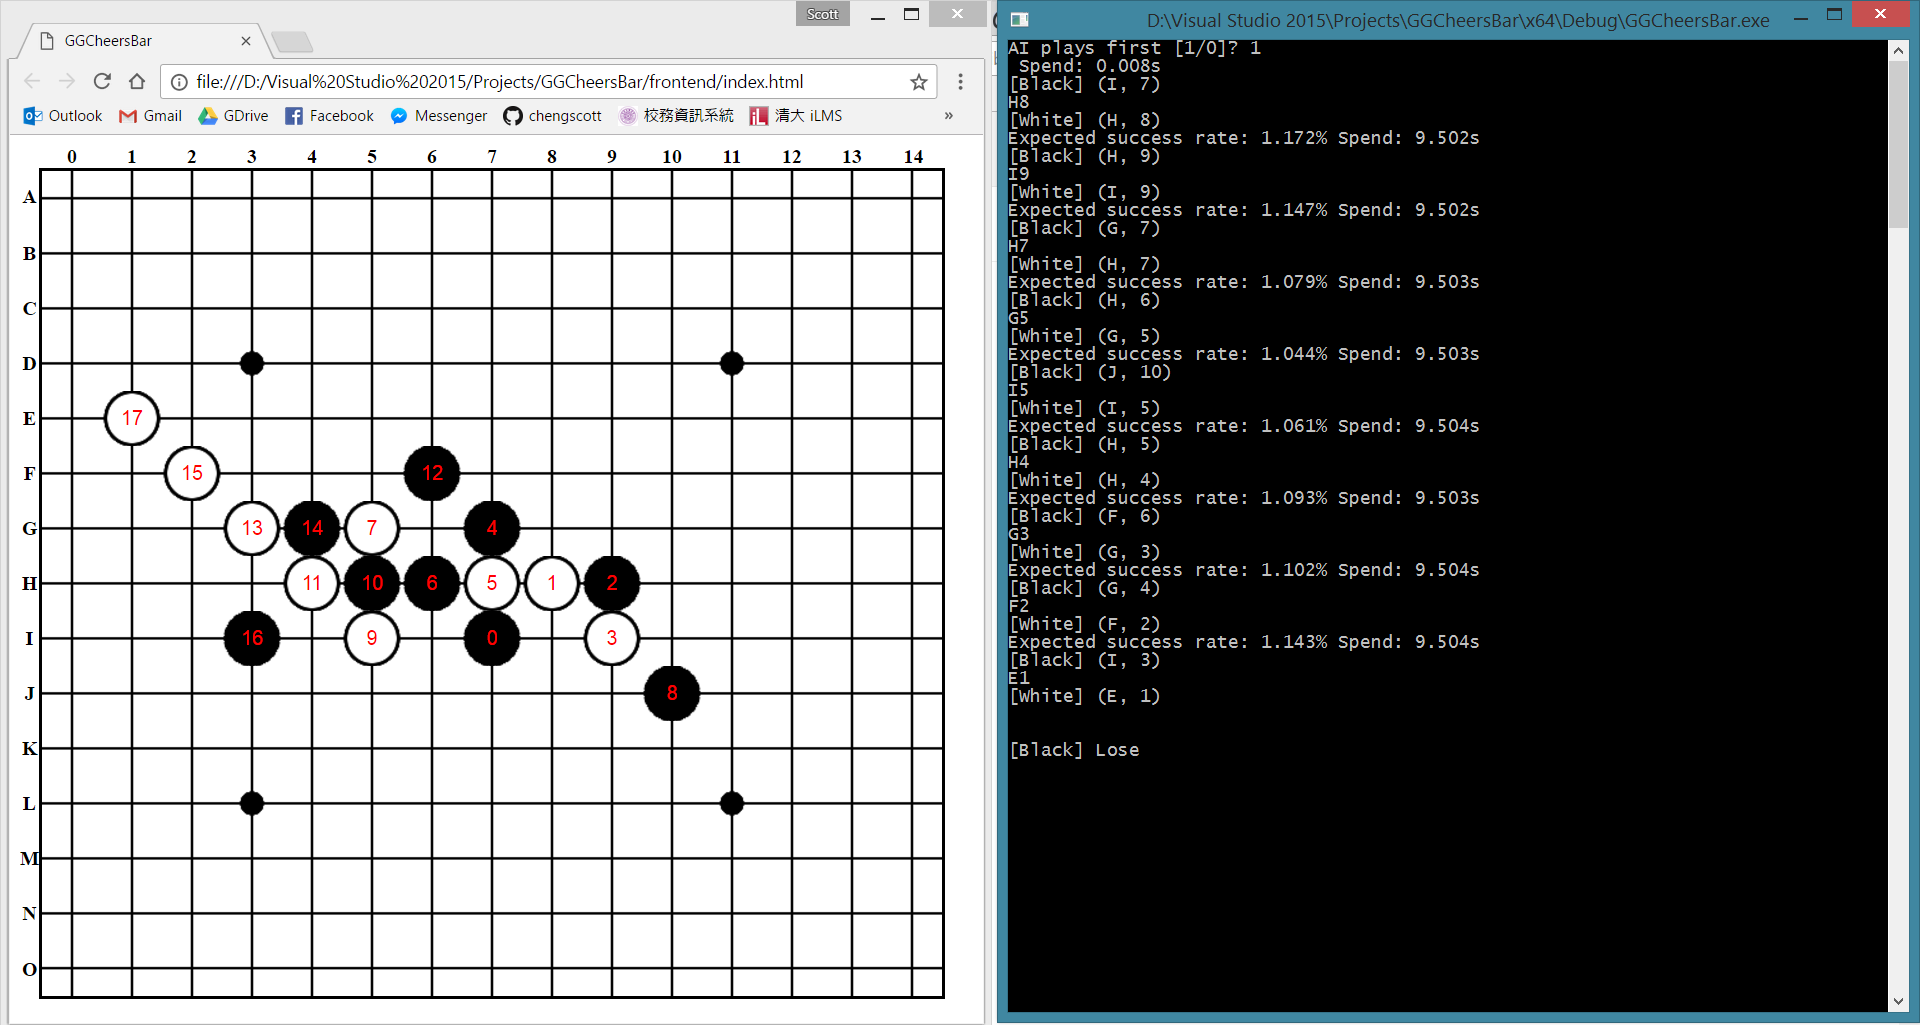
\includegraphics[width=1\textwidth]{intelligent}
\end{figure*}

\section{效能調校}
多線程、線段樹

\begin{figure*}
  \caption{計算資源}
  \centering
  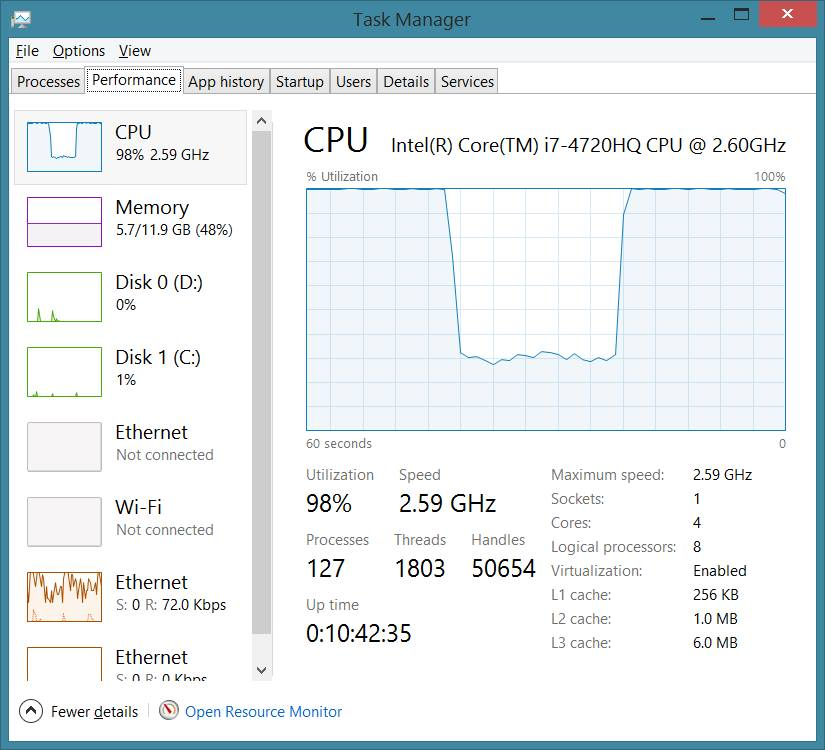
\includegraphics[width=1\textwidth]{cpu}
\end{figure*}

\begin{figure*}
  \caption{效能瓶頸}
  \centering
  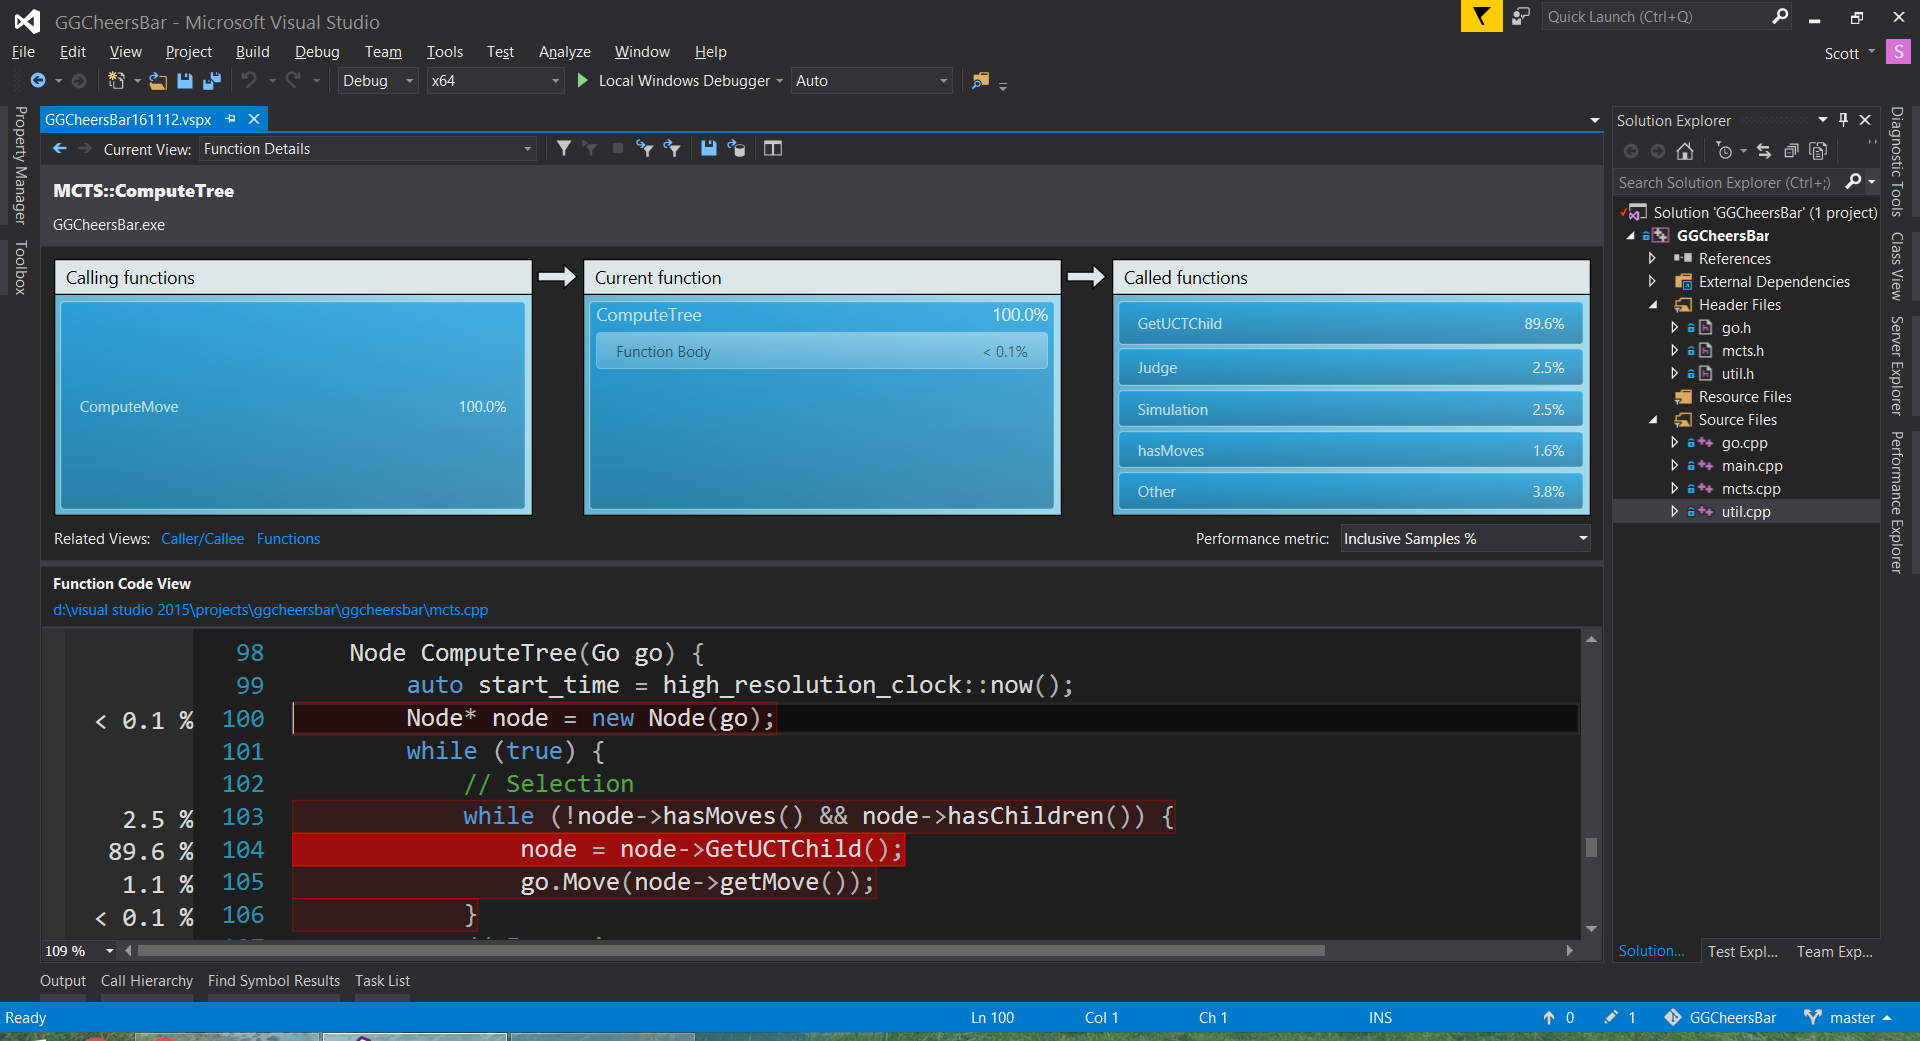
\includegraphics[width=1\textwidth]{performance}
\end{figure*}

\end{CJK}
\end{document}
